\section{Experiments}
\label{sec:experiments}
\label{sec:usecases}

We evaluate the algorithm of Section~\ref{sec:solution} on two questions.
First, are the explanations it releases useful: do they tell an analyst something about the difference between $Q$ and $Q'$ that the two queries and the constraint do not already say?
Second, what does privacy cost, in explanation quality and in running time?
Section~\ref{subsec:exp-setup} describes the data, the nine query pairs, the defaults and the baselines.
Section~\ref{sec:usecase-results} walks through one query-refinement and one CQA scenario from the constraint to the released histograms.
Section~\ref{subsec:exp-analysis} then measures accuracy against the baselines and running time.

% ---------------------------------------------------------------
\subsection{Experiment Setup}
\label{subsec:exp-setup}

\paragraph{Datasets.}
\emph{Adult} is the UCI census extract, $N=48{,}842$ tuples with demographic and employment attributes (education, occupation, hours per week, marital status, race, gender, and a binary income flag).
\emph{Tax} is the synthetic tax benchmark used in the data-cleaning literature, $N=500{,}000$ tuples with attributes such as state, marital status, number of children, salary and tax rate.
\emph{StackOverflow} is the Developer Survey, with attributes such as years of professional coding, remote-work status, company size, country, languages and AI-tool usage.
\alon{TODO: fill in $N$ and the number of explanation attributes for StackOverflow, and state which survey year is used. Everything in the repository for this dataset, and for IPUMS-CPS, was produced on a synthetic generator, not on the downloaded survey, so no StackOverflow number below may be quoted until it is re-run on the real file.}
For the CQA scenario we use the \emph{Hospital} dataset from the repair literature~\cite{rekatsinas2017}, which violates the functional dependencies $\texttt{HospitalName}\rightarrow\texttt{ZipCode}$, $\texttt{HospitalName}\rightarrow\texttt{PhoneNumber}$ and $\texttt{ZipCode}\rightarrow\texttt{City}$.
Numeric attributes are bucketed into six quantile bins, and views are conjunctions of at most two atomic conditions ($\ell\le2$).

\paragraph{Query pairs.}
Table~\ref{tab:query-pairs} lists the nine pairs, three per dataset.
In every refinement pair $Q$ violates a representation constraint and $Q'$ satisfies it, so the pairs are the output of a refinement system and not hand-picked contrasts.
The StackOverflow pairs are contrasts between two subpopulations rather than refinements; they test the framework on the setting where the two outputs are semantically far apart.

\begin{table*}[t]
\centering
\small
\caption{The nine query pairs. Shares are on the real data. Cells marked TBD are not available in the repository and need a run.}
\label{tab:query-pairs}
\begin{tabular}{@{}llp{4.6cm}p{4.6cm}l@{}}
\toprule
ID & Data & $Q$ & $Q'$ & Constraint (share $Q\rightarrow Q'$)\\
\midrule
A1 & Adult & \texttt{occupation='Craft-repair' AND hours$\ge$40} & \texttt{hours$\ge$40} & $\ge25\%$ female ($4.7\%\rightarrow26.9\%$)\\
A2 & Adult & \texttt{education IN (Bachelors, Masters) AND hours$\ge$50} & \texttt{education=Masters AND hours$\ge$30} & $\ge25\%$ female ($19.5\%\rightarrow30.6\%$)\\
A3 & Adult & TBD & TBD & TBD\\
T1 & Tax & \texttt{MaritalStatus='M' AND Rate$\le$5} & \texttt{Rate$\le$5} & $\ge30\%$ HasChild ($3.5\%\rightarrow50.1\%$)\\
T2 & Tax & TBD & TBD & TBD\\
T3 & Tax & TBD & TBD & TBD\\
S1 & StackOv. & \texttt{YearsCodePro$\ge$10} & \texttt{YearsCodePro$<$4} & contrast\\
S2 & StackOv. & \texttt{WorkRemote='Fully remote'} & \texttt{WorkRemote='On-site'} & contrast\\
S3 & StackOv. & \texttt{JobSat$>$5 AND UsingAI='Yes'} & \texttt{JobSat$>$5 AND UsingAI='No'} & contrast\\
\bottomrule
\end{tabular}
\end{table*}

\alon{Check that A1 is the pair the earlier drafts called ``Adult 6.7'' (the real counts match a craft-repair, full-time query, but the repository only keeps the label). T1 was called ``Tax 6.6''. A3, T2 and T3 do not exist in the repository as real-data runs; pick them so that each dataset has one pair whose result is surprising and one where the explanation is a sanity check.}

\paragraph{Default Parametes.}
Unless stated otherwise: $k=5$ explanations, diversity $\lambda=0.5$, total budget $\epsilon=1$ split equally between view selection, explanation selection and histogram release, $\tau=\min(3k,|\mathcal P|)=15$ views kept by the first stage, and $\gamma=2\ln(\tau|\Attrs|)\,k/\epsilon_S\approx150$ (Eqs.~\eqref{eq:tau-rule}, \eqref{eq:gamma-rule}).
Both $\tau$ and $\gamma$ are computed from public quantities and need no tuning.
Equal budget shares are not arbitrary: no allocation we swept dominates them, and starving the view stage is the one clearly bad choice, since the explanation stage can only choose among views that survive the first (at $(0.10,0.55,0.35)$ the approximation ratio on A2 falls from $0.89$ to $0.57$).
Reported quantities average $40$ trials, because the trial-to-trial standard deviation of the set score is often comparable to its mean.
\alon{TODO: all quality and runtime numbers below were produced with $\tau=35$ and $\gamma=\lceil0.005N\rceil$ ($244$ on Adult, $2{,}500$ on Tax). Re-run under the rules above. A first look at A2, scored on a fixed yardstick, put the new setting ahead of the old one.}

\paragraph{Baselines.}
No prior system explains the difference of two query outputs privately, so, as in DPXplain, we compare against reference points that each remove one ingredient of the algorithm.
All baselines are scored with the same yardstick, the set-level objective $F_\lambda$ (Def.~\ref{def:setobj}) with unsmoothed $\HD$ ($\gamma_{\mathrm{eval}}=0$). Smoothing is a device of the mechanism, and letting it define the metric would make the comparison circular.
Our metric is the ApproxRatio, the score of the released set divided by the score of the baseline's set.
\begin{description}
  \item[B1: $\epsilon\to\infty$.] The same algorithm with noise made negligible. The ratio to B1 isolates the price of noise, with the architecture held fixed.
  \item[B2: exhaustive optimum.] Scores every size-$k$ subset of candidates with $F_\lambda$ and returns the best, non-privately. The full space ($\binom{350}{5}\approx5\times10^{11}$) is not enumerable, but the optimum is computed exactly on the top-$k$ candidates of each attribute: a set that used a candidate outside the top $k$ of its attribute could swap in an unused, higher-scoring one without lowering $F_\lambda$. This leaves $50$ candidates and $\binom{50}{5}\approx2.1\times10^{6}$ subsets.
  \item[B3: non-private greedy.] Keeps the top-$\tau$ views by $\Use$ and then picks $k$ explanations greedily, with no noise anywhere.
\end{description}
B2 and B3 differ from the private algorithm in two ways at once (no noise, no private view filter), so the gap to them is the total price of privacy; the gap to B1 is the part due to noise alone.

% ---------------------------------------------------------------
\subsection{Case Studies}
\label{sec:usecase-results}

Each case follows the same five steps: the scenario and why the user needs an explanation, what the two queries already tell them, which views the first stage keeps, which explanations the second stage picks, and what the released histograms say. All released objects are produced under $\epsilon=1$; nothing else touches the data.

\subsubsection{Query refinement: hiring-style fairness on Adult (A2)}
\label{subsec:case-refinement}

\paragraph{Scenario.}
An analyst studies the share of high earners among highly educated people who work long hours:
\texttt{education IN ('Bachelors','Masters') AND hoursPerWeek >= 50}.
A representation constraint requires at least $25\%$ women, and the result has $19.5\%$ ($|Q|=3{,}055$).
A refinement system returns \texttt{education='Masters' AND hoursPerWeek >= 30}, which has $30.6\%$ women ($|Q'|=2{,}453$).
The constraint is now met, and the analyst has to decide whether the new query still asks the same question.

\paragraph{What the user can see without our framework.}
Two numbers move: women $19.5\%\rightarrow30.6\%$, and the result size goes down although the hours threshold was lowered. That tells the analyst that the education filter, not the hours filter, dominates the change. It does not tell them \emph{who} was swapped out and who came in.

\paragraph{Stage 1: views.}
Of the $1{,}052$ candidate views the algorithm keeps $\tau=15$. The view \texttt{education='Masters'} ranks $13$th on the usefulness score (coverage $0.068$, representativeness $0.53$ out of a ceiling of $3/4$) and survives.
\alon{Insert the full list of the retained views, and whether they match the exact top-15, once the view-stage experiment of Section~\ref{subsec:exp-analysis} is run.}

\paragraph{Stage 2 and release.}
Figure~\ref{fig:rel-adult-edu} shows the released explanations.
\begin{figure*}[t]
\centering
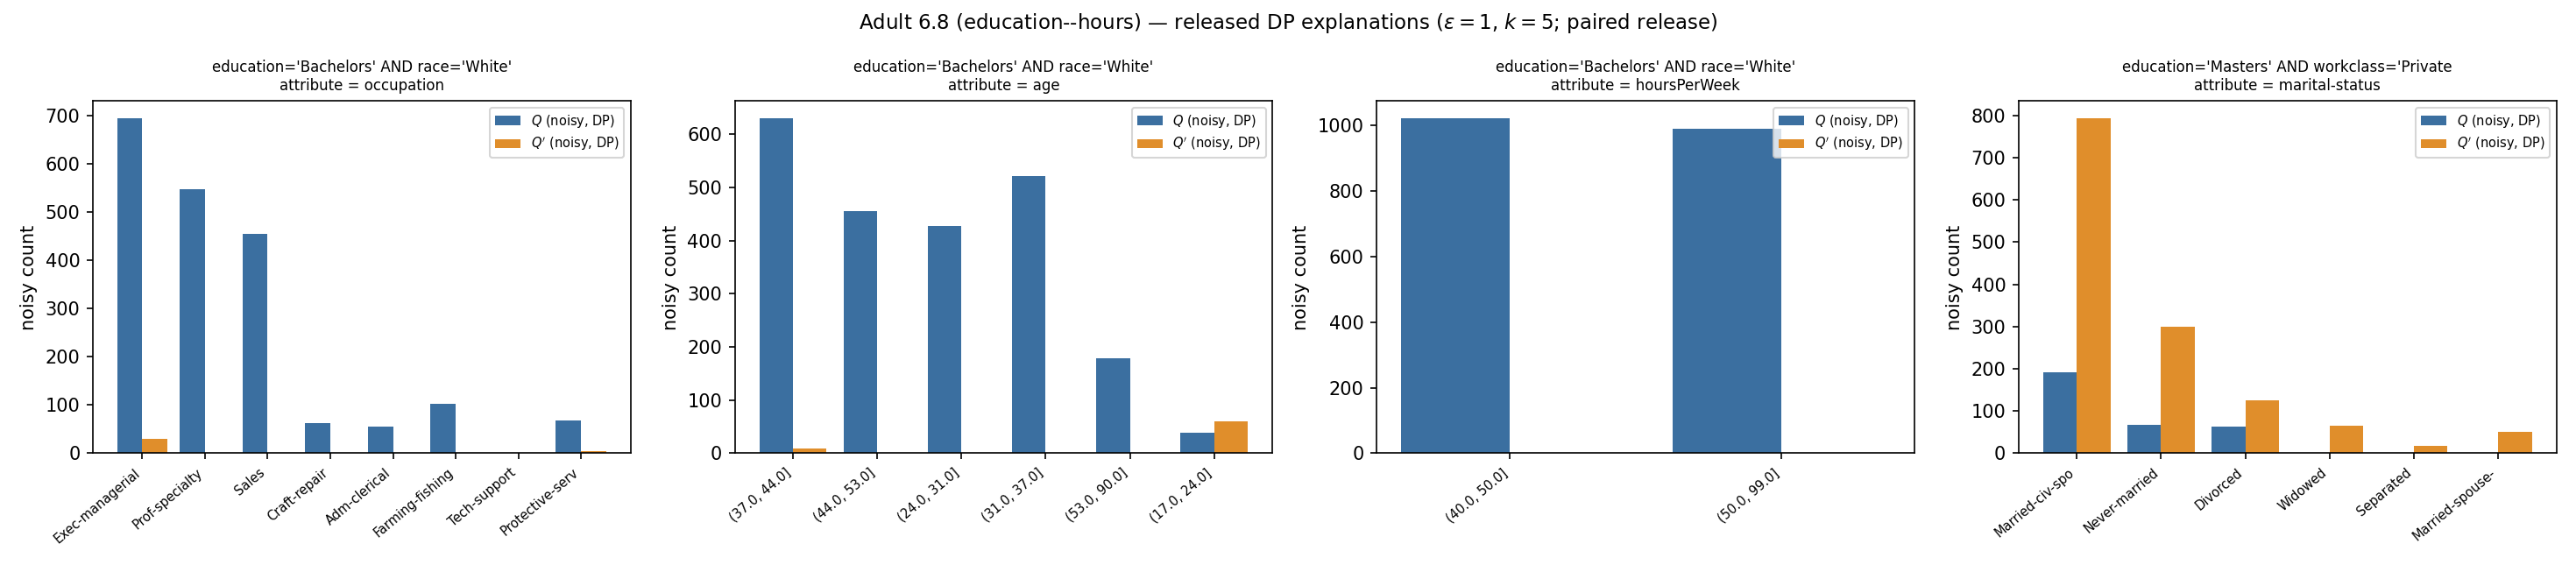
\includegraphics[width=\linewidth]{figures/U2_released_adult_education_hours.png}
\caption{A2: released $\epsilon=1$ explanations (paired release, two independently noised bars per bin). Blue is $Q$, orange is $Q'$.}
\label{fig:rel-adult-edu}
\end{figure*}
Three of the four panels sit on \texttt{education='Bachelors' AND race='White'}, the population the refinement drops. Within it, the released counts say that what is lost is a specific kind of worker: it is dominated by executive-managerial, professional-specialty and sales occupations, it is spread across all age buckets from $24$ to $53$ and not concentrated in one, and it is split evenly between the 40--50 and 50+ hour buckets.
The fourth panel is on the side of the people who come in. Within Masters degree holders in the private sector, $Q'$ adds mostly married-civilian-spouse people ($\approx790$ against $\approx190$ in $Q$), then never-married and divorced.

\paragraph{Bottom line.}
The refinement did not fix the representation of women by finding more women among the same kind of worker. It traded a population of Bachelors-level managers and professionals working $50{+}$ hours for a smaller Masters-level population with a much more married profile, which is a change of \emph{kind}, and the analyst may well not want the second population. The constraint and the sizes alone cannot show that, and the occupation view in particular tells the analyst that the high-income managerial concentration that motivated the original query has left the result.
\alon{Verify against the real histograms before submission: the figure is from a single run, the occupation claim reads off the first panel, and the claim about married people should be checked against the percentages of the female/male split inside that panel, since that is what links it to the constraint. If it does not link, drop the sentence.}

\subsubsection{Query refinement: removing a predicate on Tax (T1)}
\label{subsec:case-tax}

\paragraph{Scenario.}
An analyst studies low-rate taxpayers who are married: \texttt{MaritalStatus='M' AND Rate <= 5}.
A representation constraint requires at least $30\%$ of the result to have children (\texttt{HasChild='Y'}), and the result has only $3.5\%$.
A refinement system drops the marital-status predicate, and $Q'=\texttt{Rate <= 5}$ has $50.1\%$ \texttt{HasChild='Y'}.
The constraint is met by a wide margin, and the analyst has to decide whether the result is still the group they meant to study.

\paragraph{What the user can see without our framework.}
Everything the analyst can read off the two queries: the result roughly doubled, and the share of taxpayers with children went from $3.5\%$ to $50.1\%$. The queries also say which predicate was removed, so the identity of the new population (single filers, among others) is not news. What the analyst cannot see is what the added taxpayers look like, and why the share of parents jumped by far more than a ``more people'' change would explain.

\paragraph{Stage 1: views.}
\alon{TODO: report how many of the $\tau=15$ retained views are conditioned on \texttt{MaritalStatus='S'}, and the rank of that view by $\Use$. This is the Tax counterpart of the ``Masters ranks 13th'' sentence in A2, and is not in the repository.}

\paragraph{Stage 2 and release.}
Figure~\ref{fig:rel-tax} shows the released explanations.
\begin{figure*}[t]
\centering
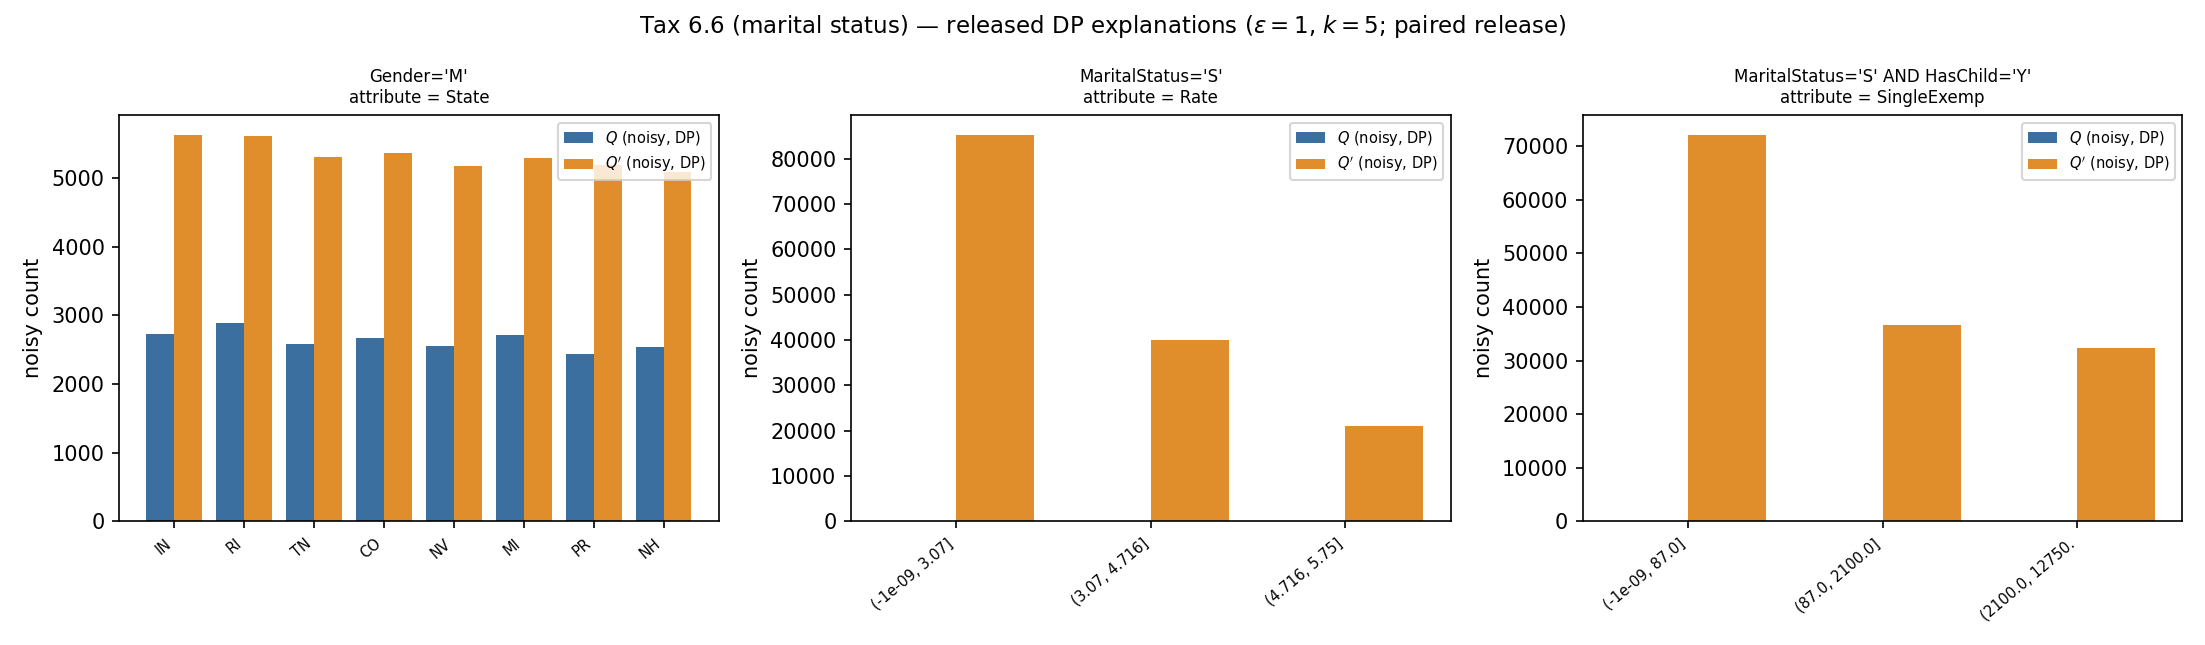
\includegraphics[width=\linewidth]{figures/U2_released_tax_marital.png}
\caption{T1: released $\epsilon=1$ explanations (paired release). Blue is $Q$, orange is $Q'$.}
\label{fig:rel-tax}
\end{figure*}
Two of the three panels sit on single filers, the population the dropped predicate introduces ($Q$ contains none, by construction). The first shows that this added population is concentrated at the bottom of the rate scale: about $85{,}000$ of the roughly $146{,}000$ added single filers fall in the lowest \texttt{Rate} bucket, and the share falls off steadily in the two higher buckets.
The second panel, restricted to single filers \emph{with children}, is the informative one. Its three bins sum to about $140{,}000$, almost the whole added population, so nearly every single filer the refinement adds has a child. The third panel, on \texttt{Gender='M'}, shows $Q'$ roughly twice $Q$ in every state, with no state standing out.

\paragraph{Bottom line.}
The refinement is described as ``drop the marital-status filter'', but what it adds is not single filers in general, it is single parents, and mostly low-rate ones. The constraint is satisfied because the added population is almost entirely made of the group the constraint asks for, not because the result became more balanced. An analyst who intended to keep studying a broad low-rate population would learn from this that $Q'$ is really a different group, and that its geographic profile is unchanged. The sanity-check part, that single filers are recovered without being told the predicate, is the part the analyst could have guessed; the single-parent composition is not.
\alon{Verify before submission: the $\approx 96\%$ figure comes from adding the three bars of the second panel and dividing by the size of the added population, so it is read from noisy counts of a single run. Compute it from the exact (non-private) histograms for the text, and report the noisy value next to it so the reader sees the release preserves it. If the exact share is much lower, rewrite the bottom line.}

\subsubsection{Consistent query answering: Hospital}
\label{subsec:case-cqa}

\paragraph{Scenario.}
On the Hospital data, the analyst aggregates, for example, the number of hospitals per state or per \texttt{HospitalType}. The data violates the three dependencies above, so the answer is computed over a repair. The pair is $(Q(D),Q_\Sigma(D))$: the same query on the inconsistent data and on its repair.
The user needs to know where the repair changed the answer and whether it did so evenly.
\alon{TODO: this case does not exist in the repository.}

\paragraph{Bottom line (to be filled).}
One sentence that says which part of the answer the repair changed and what the analyst should do about it.

% ---------------------------------------------------------------
\subsection{Accuracy and Performance Analysis}
\label{subsec:exp-analysis}

\subsubsection{Accuracy}
\label{subsec:quality}

\begin{table}[t]
\centering
\small
\caption{ApproxRatio against each baseline, $\epsilon=1$ and $\epsilon=5$, $40$ trials.}
\label{tab:quality}
\begin{tabular}{@{}lcccccc@{}}
\toprule
& \multicolumn{3}{c}{$\epsilon=1$} & \multicolumn{3}{c}{$\epsilon=5$}\\
\cmidrule(lr){2-4}\cmidrule(lr){5-7}
Pair & B1 & B2 & B3 & B1 & B2 & B3\\
\midrule
A1 & 0.883 & 0.875 & 0.875 & 0.950 & 0.941 & 0.941\\
A2 & 0.691 & 0.612 & 0.612 & 0.950 & 0.842 & 0.842\\
T1 & 0.931 & 0.901 & 0.901 & 0.995 & 0.963 & 0.963\\
\bottomrule
\end{tabular}
\end{table}

\begin{figure*}[t]
\centering
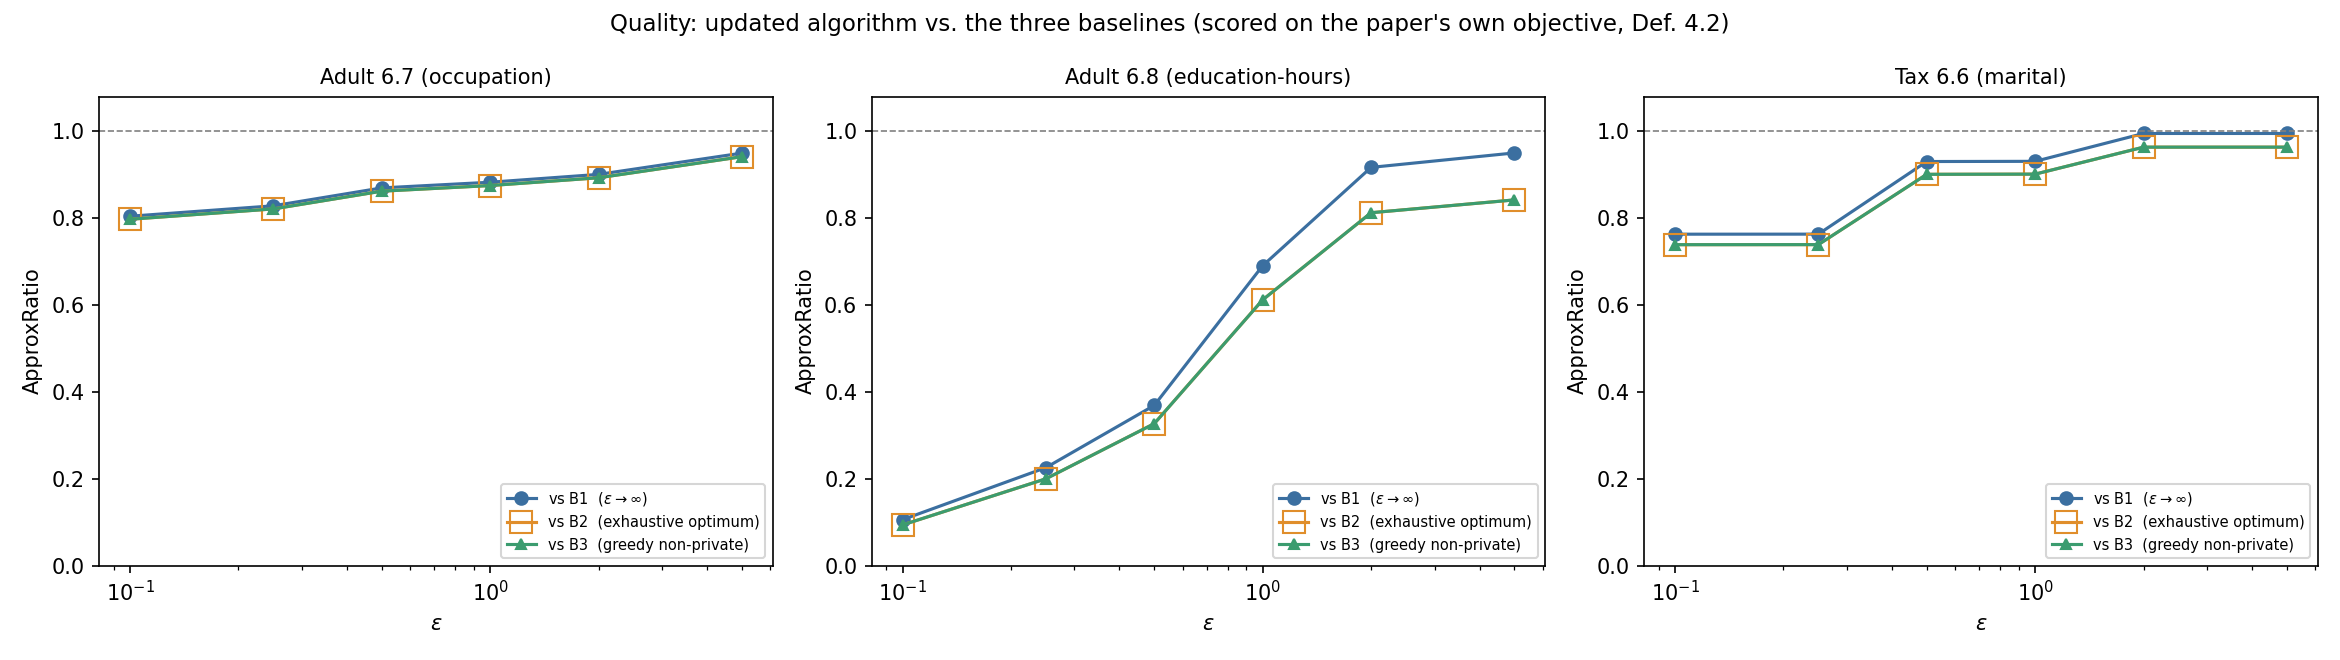
\includegraphics[width=\linewidth]{figures/Q1_approxratio_vs_baselines.png}
\caption{ApproxRatio against each baseline as a function of $\epsilon$ (scored at $\gamma_{\mathrm{eval}}=0$).}
\label{fig:quality}
\end{figure*}

At the default budget the released set reaches $0.88$--$0.93$ of the noise-free score on A1 and T1 and $0.88$--$0.90$ of the exhaustive optimum (Table~\ref{tab:quality}). Three things in the data are worth explaining.

\paragraph{The hard pair is hard because its candidates are close, not because it is small.}
A2 has the lowest ratio ($0.69$ against B1 at $\epsilon=1$, $0.11$ at $\epsilon=0.1$), while T1, with ten times the data, is the easiest. The exponential mechanism separates two candidates only if their utilities differ by more than about $2\,\Delta u\ln|C|/\epsilon_S$. On A2 the gap between the leading candidates (the \emph{margin}) is $0.027$, against $0.121$ on A1 and $0.315$ on T1, so the mechanism has almost nothing to latch onto. The margin, not $N$, is what predicts difficulty, and it is a property of the query pair rather than of the data size.

\paragraph{Greedy is the optimum, so the private gap is entirely privacy.}
B2 and B3 coincide to the last digit on all three pairs, as Proposition~\ref{prop:greedy-exact} predicts. This matters for how Table~\ref{tab:quality} is read: the remaining gap to B3 cannot be blamed on the greedy order of selection, only on noise and on the private view filter. The ratio to B2/B3 sits below the ratio to B1 by $0.01$--$0.11$, and that difference is the cost of filtering views privately; it is largest on A2, which fits the view-stage observation in Section~\ref{subsec:exp-setup} that the budget cannot be taken away from that stage.
\alon{TODO (experiment to add): the view stage in isolation. For each pair and $\epsilon_P$, the overlap of the privately retained $\tau$ views with the exact top-$\tau$ by $\Use$, and the lowest $\Use$ retained against the true $\tau$-th best. A first look at A2 suggests the overlap is low at the budgets used here and rises sharply with $\epsilon_P$, which would be the direct evidence for the claim above.}

\paragraph{Smoothing has to be matched to the bins, not to $N$.}
$\gamma$ competes with the size of individual histogram bins, and these differ far more than $N$ does: the median non-empty bin holds $20$ tuples on Adult and $3{,}897$ on Tax, a factor of $200$ for a factor of $10$ in $N$. With $\gamma$ at $0.5\%$ of $N$, it exceeds the bin count for $84\%$ of Adult bins but $30\%$ of Tax bins, and at $5\%$ of $N$ it exceeds $98\%$ and $94\%$, where $\HD_\gamma$ no longer measures relative change at all. The margins above imply a required $\gamma$ of about $292$, $66$ and $25$ for A2, A1 and T1: an ordering that is the reverse of dataset size. This is the reason $\gamma$ is derived from $\tau$, $|\Attrs|$ and the budget (Eq.~\eqref{eq:gamma-rule}) and not from $N$.
\alon{Re-check this paragraph after the rerun: it was measured under the old $\gamma$ rule and may be partly superseded.}

\subsubsection{Performance}
\label{subsec:scalability}

\begin{figure*}[t]
\centering
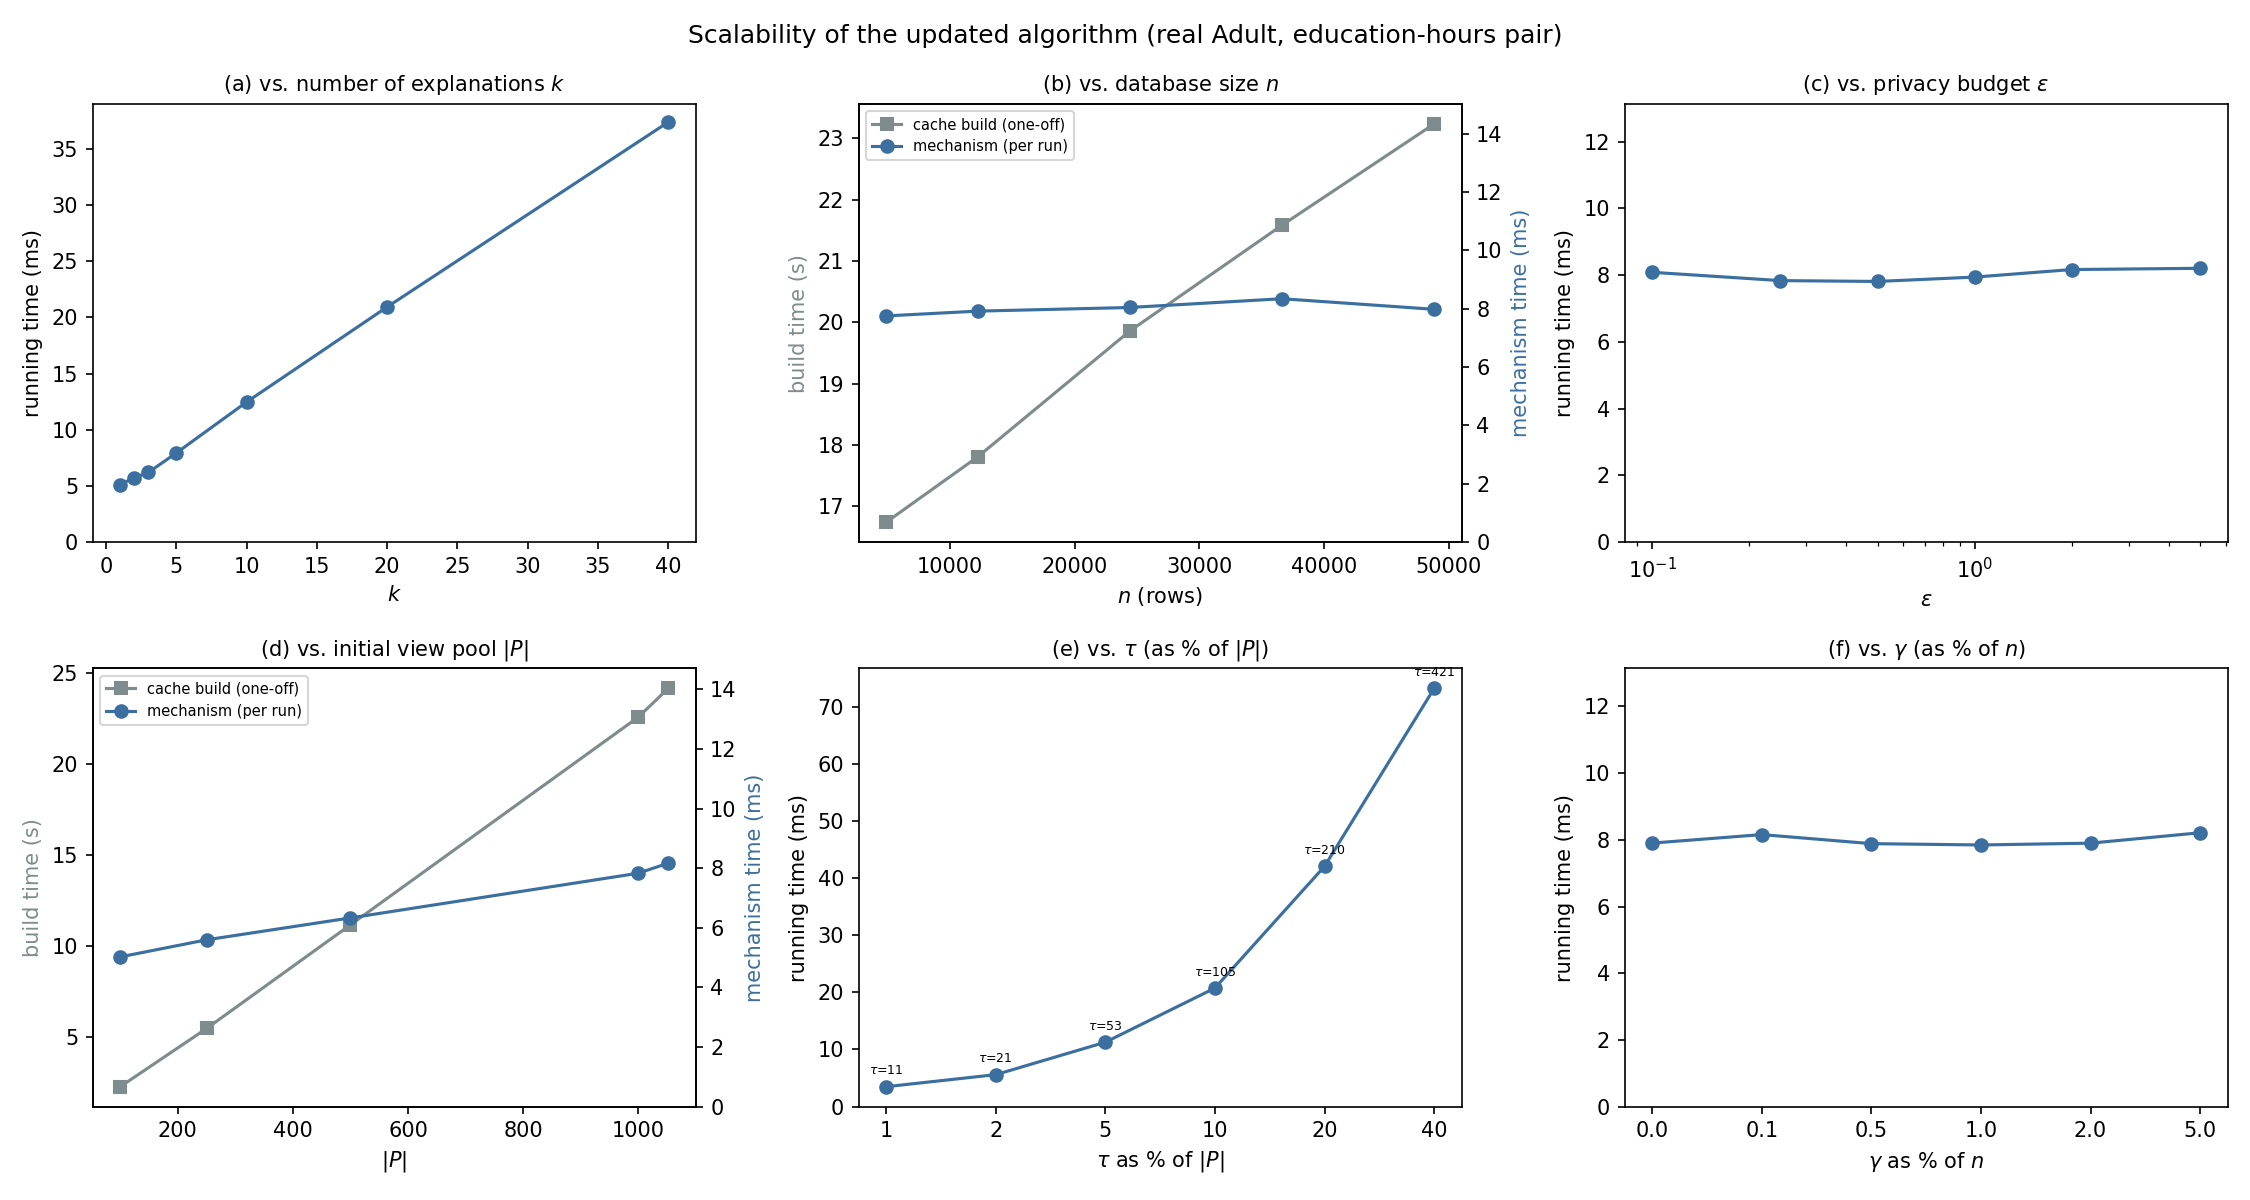
\includegraphics[width=\linewidth]{figures/S1_scalability_grid.png}
\caption{Running time of the algorithm. Panels (b) and (d) separate the one-off cache build from the per-invocation cost.}
\label{fig:scalability}
\end{figure*}

The per-invocation cost is linear in $k$ ($4.6$\,ms at $k=1$ to $36.3$\,ms at $k=40$) and in $\tau$, and flat in $N$ ($7.7$--$8.3$\,ms over a tenfold range). The reason is the structure of Section~\ref{subsec:complexity-analysis}: all the $O(N)$ work sits in the one-off preprocessing ($16.7$\,s rising to $23.2$\,s over the same range), and the $k$ selection rounds only touch the $\tau|\Attrs|$ cached scores. The same cache makes $\gamma$ free to change, and the running time is unaffected by $\epsilon$ ($7.8$--$8.2$\,ms for $\epsilon\in[0.1,5]$), so a user can re-run at a different budget interactively.

\begin{figure}[t]
\centering
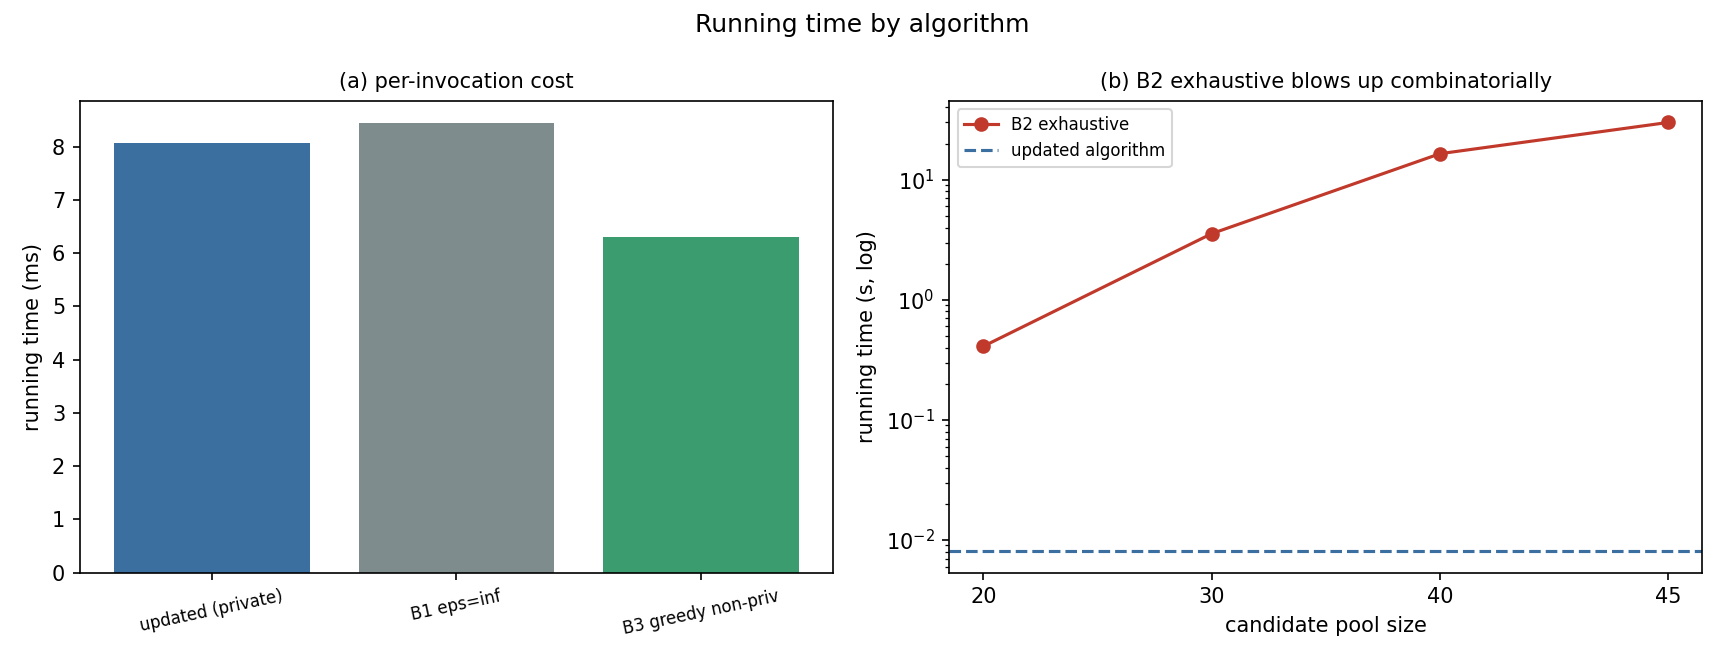
\includegraphics[width=\linewidth]{figures/S2_runtime_by_algorithm.png}
\caption{Per-invocation cost of each method, and the growth of B2.}
\label{fig:runtime-algorithm}
\end{figure}

Privacy is practically free in time: the private algorithm takes $8.1$\,ms, B1 $8.4$\,ms and B3 $6.3$\,ms. The exponential mechanism replaces an $\arg\max$ over the same scores. B2 is different in kind, growing from $0.41$\,s at $20$ candidates to $30$\,s at $45$, a $73\times$ increase for a $2.25\times$ larger pool, and taking $57$\,s on the $50$-candidate pool. The private algorithm therefore returns the same quality of set that the exhaustive search would, up to the privacy gap above, about four orders of magnitude faster.
\alon{TODO: runtime of the CQA and StackOverflow pairs, and an end-to-end time including the one-off cache build per pair, for the table.}
